\documentclass[acmsmall,review,anonymous]{acmart}\settopmatter{printfolios=true,printccs=false,printacmref=false}
\acmJournal{PACMPL}
\acmVolume{1}
\acmNumber{OOPSLA} % CONF = POPL or ICFP or OOPSLA
\acmArticle{1}
\acmYear{2018}
\acmMonth{1}
\acmDOI{} % \acmDOI{10.1145/nnnnnnn.nnnnnnn}
\startPage{1}
\setcopyright{none}
\bibliographystyle{ACM-Reference-Format}
\citestyle{acmauthoryear}   %% For author/year citations
\usepackage{my_style}
\usepackage{listings, wrapfig,xspace}
\usepackage{paralist}
\usepackage{booktabs} % To thicken table lines

\lstset{language=R}
\definecolor{LightGray}{rgb}{.92,.92,.92}
\definecolor{Gray}{rgb}{.3,.3,.3}
\definecolor{DarkGray}{rgb}{.5,.5,.5}
\lstset{ %
  columns=flexible,
  captionpos=b,
  frame=single,
  framerule=0pt,
  tabsize=2,
  belowskip=0.5em,
  backgroundcolor=\color{LightGray},
  basicstyle=\small\ttfamily,
  emphstyle=,
  keywordstyle=,
  commentstyle=\color{Gray}\em,
  stringstyle=\color{Gray},
%  numbers=left,
  showstringspaces=false
}
\lstdefinestyle{R}{ %
  language=R,
  morekeywords={assign, delayedAssign},
  deletekeywords={env, equal, c, runif, trace, args, exp, t, all},
  breaklines=true
}
\lstdefinestyle{Rin}{ %
  style=R,
  breaklines=false
}
\renewcommand{\k}[1]{{\tt #1}\xspace}


\newcommand{\eg}{\emph{e.g.},\xspace}
\newcommand{\ie}{\emph{i.e.},\xspace}
\newcommand{\cf}{\emph{cf.}\xspace}

\newcommand{\PIR}{\textsf{PIR}\xspace}
\newcommand\pirI[1]{\mathtt{#1}}
\renewcommand{\c}[1]{{\lstinline[style=Rin]!#1!}\xspace}
\newcommand{\code}[1]{{\lstinline[style=Rin]!#1!}\xspace}
% Macros for type names from the old paper.
\newcommand{\attr}[2]{\ensuremath{#1_{\mathtt{#2}}}\xspace}
\newcommand{\attrclass}[3]{\ensuremath{#1^{\mathtt{#3}}_{\mathtt{#2}}}\xspace}
\renewcommand{\to}{\ensuremath{\rightarrow}\xspace}


\renewcommand{\null}{\texttt{\textbf{null}}\xspace}
\newcommand{\any}{\texttt{\textbf{any}}\xspace}
\newcommand{\environment}{\texttt{\textbf{envir}}\xspace}
\newcommand{\expression}{\texttt{\textbf{expression}}\xspace}
\newcommand{\Language}{\texttt{\textbf{lang}}\xspace} %% Upper case!
\newcommand{\externalptr}{\texttt{\textbf{externalptr}}\xspace}
\renewcommand{\symbol}{\texttt{\textbf{symbol}}\xspace}
\newcommand{\pairlist}{\texttt{\textbf{pairlist}}\xspace}
\newcommand{\weakref}{\texttt{\textbf{weakref}}\xspace}
\renewcommand{\int}{\texttt{\textbf{int}}\xspace}
\newcommand{\chr}{\texttt{\textbf{chr}}\xspace}
\newcommand{\dbl}{\texttt{\textbf{dbl}}\xspace}
\newcommand{\lgl}{\texttt{\textbf{lgl}}\xspace}
\newcommand{\clx}{\texttt{\textbf{clx}}\xspace}
\newcommand{\raw}{\texttt{\textbf{raw}}\xspace}
\newcommand{\NA}{\texttt{{NA}}\xspace}
\newcommand{\VARGS}{\texttt{\textbf{...}}\xspace}
\newcommand{\T}{\ensuremath{T}\xspace}
\renewcommand{\S}{\ensuremath{S}\xspace}
\newcommand{\V}{\ensuremath{V}\xspace}
\newcommand{\A}{\ensuremath{A}\xspace}
\newcommand{\ID}{\ensuremath{ID}\xspace}
\newcommand{\F}{\ensuremath{F}\xspace}
\newcommand{\B}{\ensuremath{B}\xspace}
\newcommand{\FUN}[2]{\ensuremath{\langle #1 \rangle \rightarrow #2}\xspace}
\newcommand{\STRUCT}[1]{\texttt{\textbf{struct}}\ensuremath{\langle #1\rangle}\xspace}
\newcommand{\LIST}[1]{\texttt{\textbf{list}}\ensuremath{\langle #1\rangle}\xspace}
\newcommand{\CLASS}[1]{\texttt{\textbf{class}}\ensuremath{\langle #1\rangle}\xspace}
\newcommand{\VEC}[1]{#1\k{[]}\xspace}
\newcommand{\NAVEC}[1]{\k{\string^}\!#1\k{[]}\xspace}

\newcommand{\contractr}{{\sf ContractR}\xspace} % contractr
\newcommand{\roxygen}{{\sf Roxygen2}\xspace} % roxygen
\newcommand{\typetracer}{{\sf Typetracer}\xspace} % typetracer
\newcommand{\rdt}{{\sf R-dyntrace}\xspace}
\newcommand{\covr}{{\sf Covr}\xspace}




\begin{document}
\title{Designing Types for R, Empirically}

\newcommand{\NUMFUNCTIONS}{25,000\xspace}  %%% TODO auto-gen
\newcommand{\NUMPACKAGES}{412\xspace}  %%% TODO auto-gen
\newcommand{\PACKAGES}{412\xspace}  %%% TODO auto-gen
\newcommand{\genthat}{genthat\xspace}  %%% TODO auto-gen
\newcommand{\YEARS}{20\xspace} %%TODO fix
\newcommand{\PERCFAILEDASSERTIONS}{2.19\%\xspace}
\newcommand{\PERCFAILEDASSERTIONSWUNDEF}{2.23\%\xspace}
\newcommand{\PERCASSERTIONSUNDEF}{0.04\%\xspace}
\newcommand{\NUMPKGSEVAL}{7485\xspace} % autogenerate
\newcommand{\NUMASSERTIONS}{62,171,573\xspace} %autogenerate
\newcommand{\PROPFUNSFAILEDCHECK}{21.21\%\xspace}
\newcommand{\PROPFUNSFAILEDCHECKNOSTHREE}{15.48\%\xspace} 
\newcommand{\PROPARGSFAILINGASSERTS}{3.53\%\xspace} % autogen....
\newcommand{\PERCSUCCARG}{96.46\%\xspace}
\newcommand{\PERCSUCCFUNNOSTHREE}{84.52\%\xspace}
\newcommand{\PERCSUCCFUNS}{78.79\%\xspace}
\newcommand{\PERCCALLSBADFUNSINTESTS}{5.38\%\xspace}

\begin{abstract}
The R programming language is widely used in a variety of domains for tasks
related to data science. R was designed to favor an interactive style of
programming with minimal syntactic and conceptual overhead. This design is
well suited to interactive data analysis, but a bad firt for tools such as
compilers or program analyzers which must generate performant code or catch
programming errors.  In particular, R has no type annotations, its
operations are dynamically checked at runtime. The starting point for our
work are the twin questions, \emph{what expressive power is needed to
  accurately type R code?} and \emph{which type system is the R community
  willing to adopt?} Both questions are difficult to answer without actually
designing a type system and attempting to convince users and package
developers to try the proposed system.  The goal of this paper is to provide
data that can feed into the design process. To this end, we perform a large
corpus analysis with aim to gain insights in the degree of polymorphism
exhibited by idiomatic R code and explore potential benefits that the R
community could accrue from even a simple type system.  As a starting point,
we infer type signatures for \NUMFUNCTIONS functions from \NUMPACKAGES
packages among the most widely used open source R libraries. The signatures
use a minimal type language with only basic types, vectors and classes.  We
implement a contract checker that can be used to validate the inferred type
signatures.
\end{abstract} \maketitle

\section{Introduction}

Our community builds, improves, and reasons about programming languages.  To
make design decisions that benefit users, we need to understand our target
language as well as the real-world needs it answers. Often, we can appeal to
our intuition, as many languages are intended for general purpose
programming tasks. Unfortunately, intuition may fail when looking at
domain-specific languages as these languages designed for a specific group
of users to solve very specific needs. This is the case of the data science
language R.

R and its ancestor S were designed, implemented, and maintained by
statisticians. Originally they aimed to be glue languages for reading data
and calling statistical routines written in Fortran. Over three decades they
became widely used across many fields for data analysis and visualization.
Modern R, as an object of study, is fascinating. It is a vectorized,
dynamically typed, lazy functional language with limited side-effects,
extensive reflective facilities and retrofitted object-oriented programming
support.

Many of the design decisions that gave us R were intended to foster an
interactive, exploratory, programming style. These include, to name a few,
the lack of type annotations, the ability to use syntactic shortcut, and the
automatic conversion between data types.  While these choices have led to a
language with a low barrier to entry---many data science educational
programs do not teach R itself but simply introduce some of its key
libraries---they have also created a language where errors can go
undetected.

Retrofitting a type system to the R programming language would increase our
assurance in the result of data analysis. But, we are faced with two
challenges. First, it is unclear what would be the \emph{right} type system
for a language as baroque as R. For example, one of the most popular data
type, the \code{data.frame}, is manipulated through reflective operations --
a data frame is a table whose columns can be added or removed on the fly.
Second, but just as crucially, designing a type system that will be adopted
would require overcoming some prejudices and educating large numbers of
users.

This paper is a data-driven study of what a type system for the R language
could look like. Our intention is to eventually propose changes to the
language, but we are aware that for any changes to be accepted by the user
community they must clearly benefit the language without endangering
backwards compatibility. Our goal is thus to find a compromise between
simplicity and usefulness; any proposed type system should cover common
programming idioms while remaining easy to learn and to use.

This paper focuses on a simpler problem than an entire type system, instead,
we limit the scope of our investigation to giving types to function
signatures. In order to do this, we design a simple type language, one that
matches the R data types but omits features such as parametric polymorphism
and subtyping between user-defined data types. We then extract type
signature from execution traces of a corpus of widely used libraries.  This
allows us to see how far one can get with the simple type language and
identify limitations of our this particular design. We validate the
robustness of the extracted type signature by implementing a contact system
that weaves the types around their respective functions, and use a large
number of clients of the target packages for validation. The contract system
can be used by the R community to experiment with our type signatures and to
replace ad hoc error checking code.

To sum up, our paper makes the following main contributions:
\begin{itemize}
\item We implemented tooling to automatically extract type signatures from R
  functions and to intrument R functions with checks based on their declared
  types. The tooling is robust and scalable to the entire R language.
\item We carried out a large-scale analyis of corpus of \PACKAGES widely
  used and actively maintained libraries to extract function type signatures
  validated the robustness of the inferred type signatures against XXX
  programs that use those functions.
\item We report on the appropriateness and usefulness of a simpe type
  language for the R programming language.
\end{itemize}

Our tools are open source and publicly available on GitHub (link anonymize),
all results in this paper are reproducible and will be submitted for
artifact evaluation should this paper be accepted.
%
\section{Background} %%%%%%%%%%%%%%%%%%%%%%%%%%%%%%%%%%%%%%%%%%%%%%%%%%%%%%%%%

In this section, we will introduce related work and the R programming language.

\subsection{Related Work}

Dynamic programming languages such as Racket, JavaScript and PHP have been
extended post-facto with various static type systems.  In each case, the
type system was carefully engineered to match the salient characteristics of
the host languages and to foster a particular programming style. For
example, Typed Racket emphasizes functional programming and support the
migration from untyped to fully typed code~\cite{tf-popl08},
Hack~\cite{hack13} and TypeScript~\cite{BAT14} focus on typing
object-oriented features of PHP and JavaScript, respectively. They allow to
intersperse typed and untyped code in a fine-grained manner.

But what if the design of the type system is unclear?  \citet{tip} propose
an intriguing approach called trace typing. With trace typing, a new type
system can be prototyped and evaluated by applying the type rule to
execution traces of programs. While the appraoch has the limitation of
dynamic analysis techniques, namely that the results are only as good at the
coverage of the source code, it allows to quickly test new design and
quantify how much of a code base can be type-checked.  Other approaches that
infer types for dynamic analysis include the work of \citet{FurrAF2009} for
Ruby.

There is no previous work for the R programming language. We take
inspiration in the above mentionned works but focus on adapting them to our
target language.


\subsection{The R Programming Language} %%%%%%%%%%%%%%%%%%%%%%%%%%%%%%%%%

The R Project is a key tool for data analysis.  At the heart of the R
project is a \emph{vectorized, dynamic, lazy, functional, object-oriented}
programming language with a rather unusual combination of
features~\cite{ecoop12} designed to ease learning by non-programmer and
enable rapid development of new statistical methods.  The language was
designed~\citet{R96} as a successor to S~\cite{S88}.

In this paper, we will attempt infer type signature for functions. We now
introduce some relevant concepts.  Functions can be called with named
parameters, arguments can have default values, and R also support variable
argument lists.  To illustrate all of this in a single example, consider:

\begin{lstlisting}
  f <- function(x, ..., y=if(z==0) 1, z=0) x + y + if (missing(...)) 0 else c(...)
\end{lstlisting}

\noindent
This function four formal parameters, \k x, \k{...}, \k y and \k z. Argument
\k x can be bound positionally or passed by name. The vararg argument,
\k{...}, is always passed positionally. The remaining two arguments must be
passed by name.  Arguments \k y and \k z have default values, in the case of
\k z this is a constant, but \k{y}'s default value is an expression that
depends on the value of \k z. The body of the function will add parameters
\k x and \k y with either the scalar 0 or the result of concatenating the
varargs into a primitive vector. The function \k{missing} tests if an
argument was explicitly passed. The following are some valid invocations
of \k f:

\begin{lstlisting}
 > f(1)    
 [1] 2             % a double vector, y is 0, ... is missing
 > f(1,2) 
 [1] 4             % a double vector, y is 0, ... is 2
 > f(1,2,3)
 [1] 4 5           % a double vector, y is 0, ... is 2, 3
 > f(2,3,x=1)
 [1] 4 5           % a double vector, y is 0, ... is 2, 3
 > f(x=1, y= 1)
 [1] 2             % a double vector, y is 1, ... is missing
 > f(x=1, z= 1)
 numeric(0)        % a double vector of length 0, y is NULL
 > f(1L,2L,y=1L)
 [1] 4             % an integer vector, y is integer 1, ... is integer 2
 > f(1, y=c(1,2))
 [1] 1 2           % a double vetor, y is 1, 2, ... is missing
\end{lstlisting}

\noindent
The above hints at the polymorphism of the language, \k f, may return a
vector of integer or of double, the length of the vector depends on the
length of the varargs and of \k x and \k y.  The language does not really
differentiate between scalar and vectors.
Some more exotic types that can be encountered include vectors of complex
number and list of arbitrary types. Function \k f can be invoked with those
as well.

\begin{lstlisting}
 > c1 <- complex(re=1, im=2)
 > c2 <- complex(re=2, im=1)
 > f(c1)
 [1] 1             % a double vector, x is complex, y is double
 > f(c1,y=c2)
 [1] 2+1i          % a complex vector, x and y are complex
 > l1 <- list(1,2)
 > l2 <- list(c1,c2)
 > f(l1) 
 [1] 1             % a double vector, x is a list of doubles
 > f(l1,y=l2)
 [[1]]             % a list of complex, x is a list of doubles
 [1] 1+2i          %                      y is a list of complex
 
 [[2]]
 [1] 2+1i
\end{lstlisting}

R has one builtin notion of type that can be queried by the \k{typeof}
function. Figure~\ref{rtypes} lists all of the builtin types that are
provided by the language. They are the possible return values of
\k{typeof}. There is no intrinsic notion of subtyping in R. But, in many
context a \k{logical} will convert to \k{integer}, and an \k{integer} will
convert to \k{double}.  Some odd conversions can occur in corner cases, such
as \k{1<"2"} holds and \k{c(1,2)[1.6]} returns the first element of the
vector, as the double is converted to an integer. R does not distinguish
between scalars and vectors (they are all vectors), so \code{typeof(5) ==}
\code{typeof(c(5)) == typeof(c(5,5))} \code{ == "double"}. Finally all
vectorized data types have a distinguished missing value denoted by
\code{NA}. The default type of \code{NA} is \k{logical}. We can see that
\code{typeof(NA)=="logical"}, but NA inhabits every type:
\code{typeof(c(1,NA)[2])=="double"}.

\begin{wrapfigure}{r}{6.1cm}
\footnotesize\begin{tabular}{l|l@{}}\hline
\multicolumn{2}{l}{\bf Vectorized data types:}  \\\hline
\k{logical}   & vector of boolean values\\
\k{integer}   & vector of 32 bit integer values\\
\k{double}    & vector of 64 bit floating points\\
\k{complex}   & vector of complex values\\
\k{character} & vector of strings values\\
\k{raw}       & vector of bytes\\
\k{list}      & vector of values of any type\\\hline
\multicolumn{2}{l}{\bf Scalar data types:}\\\hline
\k{NULL}      &  singleton null value\\
\k{S4}        &  instance of a S4 class \\
\k{closure}   &  function with its environment\\
\k{environment}& mapping from symbol to value \\\hline
\multicolumn{2}{l}{\bf Implementation data types:}\\\hline
\multicolumn{2}{l}{\k{special},
\k{builtin},
\k{symbol},
\k{pairlist},
\k{promise}}\\
\multicolumn{2}{l}{
\k{language},
\k{char},
\k{...},
\k{any},
\k{expression},
}\\
\multicolumn{2}{l}{
\k{externalprt},
\k{bytecode},
\k{weakref}}\\\hline
\end{tabular}\caption{Builtin Types}\label{rtypes}\end{wrapfigure}

With one exception all vectorized data types are monomorphic, the exception
is the \k{list} type which can hold values of any other type including
\k{list}. For all monomorphic data types, attempting to store a value of a
different type will cause a conversion. Either the value is converted to the
type of vector, or the vector is converted to the type of the value.

Over the years, programmers have found the need for a richer type structure
and have added {\it attributes}. The best way to think of attributes is as
an optional map from name to values that can be attached to any object.
Attributes are used to encode various type structures. They can be queried
with functions such as \k{attributes} and \k{class}.  The addition of
attributes lets programmers extend the set of types by tagging data with
user-defined attributes. For example, one could define a vector of four
values, \code{x<-c(1,2,3,4)} and then attach the attribute \k{dim} with a
pair of numbers as value: \code{attr(x,"dim")<-c(2,2)}.  From that point,
arithmetic functions will treat \k{x} as a 2x2 matrix. Another attribute
that can be set is the \k{class}.  This attribute can be bound to a list of
class names. For instance, \code{class(x)<-"human"}, set the class of \k{x}
to be \k{human}.  Attributes are thus used for object-oriented
programming. The S3 object system support single dispatch on the class of
the first argument of a function, whereas the S4 object system allows
multiple dispatch (on all arguments). Some of the most widely used data
type, such as data frames, leverage attributes. A data frame, for instance,
is a list of vectors with a class and a column name attribute.

Scalar data types include the distinguished \k{NULL} value, which is also of
ktype \k{NULL}, instance of classes written using the S4 object system,
closures and environments.  The implementation of R has a number of other
types listed in Figure~\ref{rtypes} for reference.

%%%%%%%%%%%%%%%%%%%%%%%%%%%%%%%%%%%%%%%%%%%%%%%%%%%%%%%%%%%%%%%%%%%%%%%%%%%%%%
\section{Designing A Type Language for R}%%%%%%%%%%%%%%%%%%%%%%%%%%%%%%%%%%%%%


This section sets out to propose a candidate design for a type language that
can be used to describe the arguments and return values of functions in R.
The goal is not to be the final design but rather a starting point for an
iterative process.

Fig.~\ref{types} presents our type language. An early design choice was to
stay close to the R language and only depart in small, hopefully,
non-controverwsial ways.  Functions types have the form \FUN{A_1, \dots,
  A_n}\T where each $\A_i$ argument is either a type \T or \VARGS, a
variable length argument list. The rest of this section details and
motivates our design.

\begin{figure}[!h] \noindent \small  \centering\begin{minipage}{.45\linewidth}
\begin{tabular}{lclr}
\T& ::= & \any          & \it top type\\
  & |   & \null         & \it null type\\
  & |   & \environment  & \it environment type \\
  & |   & \S            & \it scalar type \\
  & |   & \V            & \it vector type \\
  & |   & \T~\k{|}\T    & \it union type \\
  & |   & \k{?} \T      & \it nullable type \\
  & |   & \FUN{A_1, ..., A_n}\T    & \it function type \\
  & |   & \LIST\T                  & \it list type\\
  & |   & \CLASS{ID_1, ..., ID_n}  & \it class type\vspace{5pt}\\
\end{tabular}\end{minipage}   \hfill
\begin{minipage}{.45\linewidth}\begin{tabular}{lclr}
\A & ::= & \T          & \it arguments \\
   & |   & \VARGS      & \vspace{5pt} \\
\V & ::= & ~\VEC\S     & \\
   & |   & \NAVEC\S    & \it na vector types \vspace{5pt}\\
\S & ::= & \int        & \\
   & |   & \chr \\
   & |   & \dbl \\
   & |   & \lgl \\
   & |   & \clx \\
   & |   & \raw \vspace{5pt}\\
\end{tabular}\end{minipage}\caption{The R type language}\label{types}
\end{figure}

\paragraph{Scalar vs. Vectors} Our type system distinguishes between
vectors of length 1, and vectors of any dimensions. The six base types,
integers, doubles, complex numbers, logicals (booleans), characters, and
raws (bytes), can be either vectors (e.g., \VEC\int) or scalars (e.g.,
\int).  It is worthwhile to note that a vector can happen to be of length 1
and thus a scalar value is a subtype of the corresponding vector type.
Vectors are homogeneous, in that a vector of doubles contains only doubles.

\paragraph{Missing values} In R, a missing value is written
\NA, each of basic types has its specific representation of \NA. Thus there
is an \int missing observation as well as a double missing, and they are
different.  The type system allows to distinguish between vectors that may
contain missing observations (written \NAVEC\int) and those who are
guarantee to be \NA-free (\VEC\int).  A \NA-free vector can be treated as a
vector that may have missing observations.  We do not allow scalar values to
be missings.  The type \raw does not allow {\NA}s.

\paragraph{Unions} We support untagged unions of types written
$\T_1 \k{|} \T_n$.

\paragraph{Nullables} 
The type system has a \null type that is inhabited by a singleton
\code{NULL} value. This value is often used as a sentinel or as a stand in
for arguments that were not provided.  To capture this behavior, we
introduce a nullable type \code{?}\T.  The difference between the \NA and
\code{NULL} values is that \NA can be stored in primitive vectors.

\paragraph{Lists} Heterogeneous collections are implemented using lists.
Lists and vectors are closely related. Any vector can be converted to a list
with \code{as.list}, and lists to vectors with \code{unlist} (coercions may
ensue). We support parametrization of the list type, \LIST\T, but for
heterogenous lists this type will default to \any.

\paragraph{Classes} 
R has more than one notion of type. Values can be attributed, one important
attribute is the class of a value.  A class is a list of names that are used
to mimic object-oriented programming. The type system includes class types
written \CLASS{\ID_1,\dots,\ID_n}.

\paragraph{Environments}
Environments are lists with reference semantics: mutating a value in an
environment is performed in-place.  They are used to store variables and to
escape from the copy-on-write semantics of other data types.  Environments
are comprised of name, value pairs, and each environment has a reference to
its parent environment. 

%
%
\section{Extracting and Checking Signatures}

For this paper, we have built tooling to (\emph{a}) automate the extraction
of raw type signatures from execution traces, (\emph{b}) infer type
signatures from a set of raw types, and (\emph{c}) validate the inferred
signatures by the means of contracts. This section presents each step
of this pipeline.

\subsection{Extracting raw type signature from traces}

We implemented \typetracer an automated tool for extracting raw type
signatures from execution traces of R programs. The goal of this tool is to
output a tuple $\langle f, t_1, \dots, t_n, t\rangle$ for each function call
during the execution of a program, where $f$ is an identifier for a
function, $t_i$ are type-level summaries of the arguments and $t$ is a
summary of the return value.

While this task is seemingly simple, the details and their proverbial devil
are surprisingly tricky to get right and to scale to long running programs.
To avoid starting from scratch, our implementation reuses an open source
dynamic analysis framework for R named \rdt~\cite{oopsla19} which consists
of an instrumented R Virtual Machine based on GNU-R version 3.5.0. The
framework exposes hooks at key points in the R interpreter to which user
defined callbacks can be attached. These hooks include function entry and
exit, method dispatch for the S3 and S4 object systems, the longjumps used
by the interpreter to implement non-local exit, creation and forcing of
promises (lazy evaluation), variable definition, value creation, mutation
and garbage collection.

\paragraph{Raw types}
The type information output by the tool includes the \emph{type tag} of each
value. The R internal types are translated to names in the proposed type
system. The next bit of information output is the \emph{class} which is an
optional list of names, it may be absent, and, in some cases, it may be
implicit (i.e. the interpreter blesses some values with the \k{matrix} and
\k{array} classes even when they have no attributes). 
Depending on the value's type tag, the tool collects further information:

\begin{itemize}
\item For vectors, the number of dimensions and the present of \NA values.
\item For lists, a recursive traversal collects element types.
\item For promises, we attempt to establish the type of its result or output
  \any.
\end{itemize}

\noindent
To obtain raw types, we make use of R's C FFI and use low-level machinery to
collect type tags and attributes from the R runtime.  The types that we
provide to users are constructed during post-processing, and rely on the
detailed information made available by these low-level reflection
mechanisms.

\paragraph{Varargs}
Arguments that are part of a function's varargs (denoted \VARGS) are
ignored, as type \any is output for the entire varag construct.


\paragraph{Promises}
The fact that arguments are evaluated lazily, i.e. expression are packing
into promises and evaluated on first access, complicates the information
gathering.  For example, some promises remain un-evaluated, and it would be
erroneous to force them as they may cause side-effects that will affect the
programs execution.  To deal with unevaluated arguments, we make an initial
guess for each argument at fufnction entry.  If the promise is later forced,
we simply update the recorded type for the argument.

\paragraph{Missing arguments}
Parameters which receive no values when the function is called are termed
missing. This occurs when a function was called with too few arguments and
no default value was specified for missing arguments.  We record a
\k{missing} type for such argument.  There are two obvious ways to deal with
missing arguments: type them as \any or type them as some unit type.  As we
are performing a dynamic analysis, we conservatively type them as \any.

\paragraph{Non-local returns}
When a function exits with a longjump there is no return value to speak
of. In order to ensure that call traces are valid when a longjump occurs, we
intercept the unwinding process initiated by the longjump and mimics the
functionality of the functions being exited. When no return value is present
for a call, we record a special \k{jumped} return type.

\paragraph{Implementation details.}
We primarily rely on eight callbacks: \k{closure\_entry}, \k{closure\_exit},
\k{builtin\_entry}, \k{builtin\_exit}, \k{special\_entry},
\k{special\_exit}, \k{promise\_force\_entry}, and
\k{prom\-ise\_force\_exit}.  The function-related callbacks are used mainly
for bookkeeping: the analysis is notified that a construct has been entered
by pushing the call onto a stack.  The calls themselves store a trace
object, it is that object that holds the type information. As R can perform
single or multiple dispatch on function arguments depending on their class,
the relevant information is kept by the {\tt \_entry} variants.



\subsection{Inferring type signatures from raw types}

The output of the \typetracer tool consists of a set of tuples of row types,
each representing a function call in some program's execution. The inference
step consolidate the different tuples corresponding to a particular function
definition across multiple programs and distills them into a single type
signature.  The shape of the infered function signatures is:

\medskip
\FUN{ T_{1,1} \k{~|~} T_{1,i}, \dots, T_{n,1} \k{~|~} T_{n,j}}{T_1\k{~|~} T_k}
\medskip

\noindent
In other words, we take the union of the types occurring at individual
argument positions rather than an union of function types. Furthermore we
apply some transformation on the types to keep the size of types in check.

\medskip
\begin{tabular}{rclll}
  \T \k{~|~} \T  & $\Rightarrow$ &  \T &  \\
  \T \k{~|~} $T'$ & $\Rightarrow$ &  \T & \it{iff} $T' <: T$  \\
  \LIST{\T} \k{~|~} $\LIST{T'}$ & $\Rightarrow$ &  \LIST\T & \it{iff} $T' <: T$  \\
   $\null \k{~|~} \VEC{\S_1} \k{~|~}\dots \VEC{\S_n}$  & $\Rightarrow$ &
    $ \NAVEC{\S_1} \k{~|~}\dots \NAVEC{\S_n}$ &  \\  
\end{tabular}
\medskip

\noindent
Assuming that type sequences can be reordered freely, we rewrite types to
minimize their size by removing redundant types, types that are subsumed by
subtyping, and \null types.

\subsection{Checking types signatures with contracts}

\contractr is an R package that implements our type system for the R package
ecosystem. For functions with type annotations, it adds contracts for
type-checking arguments and results on function calls. On contract failure,
it reports a type mismatch warning with the package name, function name,
argument name, argument position, expected type signature, actual type
signature of the value observed, and a stack trace for the called
function. \contractr works by modifying function definition to insert a call
to the type-checking function. When the modified function is called, the
type-checking function is invoked on the modified function's arguments and
return value.

\contractr is implemented in 434 R LOC and 2358 C++ LOC. The core
implementation is in C++ to keep the runtime overhead low. It been designed and
tested with GNU R-3.5.0 but it also works with recent versions of R. It has been
hardened with a battery of 400 test cases. We have used it extensively during
the course of this work; firstly, for sanity checking of XXX type signatures
generated for the XXX packages during the development phase, and secondly, for
assessing the quality of these type signatures on XXX packages during the
evaluation phase. We discuss this further in Section~\ref{sec:evaluation}.

%
%
\subsubsection{Type Declarations}
Type declarations can be made available to \contractr in three ways: as
part of its internal database of types (which already has type signatures for
our corpus of 500 packages), as part of a designated \emph{TYPEDECLARATION} file
supplied by the package author and installed along with the package, or through
a user-level API function insert\_contract that lets the user insert contract to
a custom function with the type declaration provided as a string argument.

%
%
\subsubsection{Challenges}
Retrofitting a robust and efficient type-system as an external package in R
has been a significant undertaking. We had to contend with the complex
design choices of R to make it work without surprises for the end-users. We
describe two key challenges that we faced in the development of \contractr.


Firstly, we faced the problem of type-checking arguments in a non-strict
language while retaining the non-strict semantics. Recall that when a
function is called in R, parameters are bound to unevaluated code thunks
called promises~\cite{oopsla19}, instead of values which can be immediately
type-checked. Naively forcing promises at function call to obtain a value
for type-checking would violate the language semantics, leading to incorrect
results. To preserve the original semantics, \contractr modifies the promise
by wrapping the unevaluated promise expression in a call to its type-checker
along with the context necessary to associate the promise to the function
and its parameter (for failure messages). The contract checking happens when
the promise is evaluated, either inside the function or many calls deep.
This works, but with one wrinkle. GNU R has a bytecode compiler that can
sometimes optimize away promises; in those cases, \contractr receives values
that can be immediately type-checked. Non-strict semantics dictate that any
computation related to the argument should happen on the first use of the
argument. So type-checking at this point and issuing an error message would
violate the non-strict semantics; if this argument is never used, it would
be incorrect to type-check it at the beginning of call. To make this work,
\contractr mutates the function parameter binding to a promise that wraps
the argument value in a call to the type-checker, as in the previous case.


Secondly, we faced the problem of type-checking function return value. In R,
the result of a function call is the result of evaluating the last
expression in the function body; so an explicit return call is absent from
most function definitions. Thus, there could be many potential
sub-expressions in the function body which need to be type-checked against
the return type. To address this, \contractr registers the type-checker to
be called on the return value through a function exit hook. This hook is
executed in the function call's environment after it has executed. While
this works, we have to contend with yet another wrinkle, R interpreter can
perform longjumps in its C implementation, which causes active R function
calls on the stack to be discarded. When they are discarded, their exit
hooks are called, which in this case calls the registered type-checker. But,
these functions are in the middle of an active computation, so they don't
have a return value to type-check. \contractr deals with this problem by
allocating a unique sentinel object which serves as the return value for
calls that are discarded. The function call exit hook does not call the
type-checker if this unique value happens to be the return value of the
call.

\subsubsection{Usability}
With \contractr, we aim to provide a hassle-free path to the R developers
for adding types to untyped package code. Hence, we have paid a lot of
attention towards usability in its design. We discuss three such usability
features.


\contractr enables automatic type-checking on importing without any user
intervention. Just running \code{library(contractr)} R code is enough to
insert contracts, both, in packages pre-loaded in the user's workspace, and,
in packages that will be loaded eventually. To achieve this automation,
\contractr relies heavily on R's reflective and dynamic capabilities. On
loading, \contractr scans all the pre-loaded packages in the user's
workspace and inserts contracts in functions for which type signatures are
available. For all other packages installed on user's machine but not yet
loaded in the workspace, \contractr sets up package load hooks which are
executed by R when those packages are loaded. The hook registered by
\contractr insert contracts to those package's functions. Thus, developers
and users do not have to call the \contractr API to enable type-checking for
packages at any point of their programming workflow. Furthermore, \contractr
automatically removes contracts from all the package functions and restores
them to their original state when it is unloaded, an operation that is
rarely performed, but useful in interactive settings.

\contractr enables package authors to supply type declarations for their
package without requiring package code modifications. Type declarations can
be written alongside a \code{@type} section inside \roxygen function comment
blocks. \roxygen is an R package that enables authors to add documentation
to R functions in the form of organized plaintext sections which are
automatically exported to R's latex style custom documentation format.
\roxygen is a widely adopted package, used by over XXX R packages in
CRAN. It provides an extension API for adding custom documentation tag
sections in comment blocks. The sections are processed by \roxygen before
package build step and a registered method for each custom tag section is
invoked with the section data and documented object. \contractr uses this
mechanism to register a hook for a custom \code{@type} tag. This hook parses
the type declarations from the \code{@type} sections, extracts the function
name from the documented function definition, and stores them in a
TYPEDECLARATION file inside the package folder. This files is copied
verbatim on package installation and picked up \contractr when the package
is loaded. Here is an example of how a roxygen code block looks like with
our type declaration:

This feature enables a function and its type signature to coexist next to
each other, where they are more likely to remain synchronized. Furthermore,
the \contractr hook can also add the function's type declaration to its
documentation, which seamlessly integrate our type system with the existing
R tooling.
  
\contractr provides a very expressive API to the users, covering a variety
of uses cases. During interactive development, developers can explicitly
insert contracts by supplying the type declaration as a string argument to
the \code{insert\_contract} API function. Conversely, contracts can be
removed by calling the \code{remove\_contract} API on functions. Contracts
can be selectively enabled or disabled for code blocks by wrapping them in
calls to \code{ignore\_contracts} and \code{capture\_contracts}
functions. This enables selective type-checking of code section during the
development phase.  Furthermore, these functions return a data frame that
contains all the information about failed and successful contract assertions
in the wrapped code blocks. This is useful for post-hoc
investigation. Multiple type-checking failures can introduce a lot of noise
in the program output. To alleviate this problem, \code{contractr.severity}
option can be set to \code{'silence'}.  This suppresses failure messages but
\contractr still performs type-checking whose results can be explicitly
obtained as a data frame from the \code{get\_contracts} API function. R
suppresses printing of warnings on the terminal when a function issues too
many warnings. This can hide type-checking failure messages. Setting
\code{contractr.severity} flag to \code{'error'} turns the type-checking
failure warnings to errors, which halts the program at the point of contract
failure.


While \contractr's primary logic has been implemented in C++, we have not
observed a single segfault during our use of the package, either during the
development and sanity-checking phase, or during the evaluation phase.
We conclude the discussion of \contractr by drawing reader's attention to the
engineering effort it takes to package experimental ideas in the form of stable
and easy-to-use tools. R has an eclectic mix of features and design oddities
that make this even harder. 


%
%%%%%%%%%%%%%%%%%%%%%%%%%%%%%%%%%%%%%%%%%%%%%%%%%%%%%%%%%%%%%%%%%%%%%%%%%%%%%
\section{Project Corpus}\label{sec:corpus} %%%%%%%%%%%%%%%%%%%%%%%%%%%%%%%%%%

For this paper we have selected \CorpusLoadable packages consisting of
\CorpusRCodeRnd lines of R code and \CorpusNativeCodeRnd lines of native
code (C/C++/Fortran). Figure~\ref{fig:corpus} shows all the packages, the
size of the dots reflects the size of the project in terms of both R and
native lines of code\footnote{ Lines of source code reported excludes
  comments and blank lines, counted by \emph{cloc}, \cf
  \url{https://github.com/AlDanial/cloc}}, the x-axis indicates the
expression code coverage in percents and the y-axis gives the number of
reverse dependencies in log scale. Dotted lines indicate means.  Packages
with over \PackageSizeOutierRnd lines of code are annotated.

\begin{figure}[!h]  \centering
  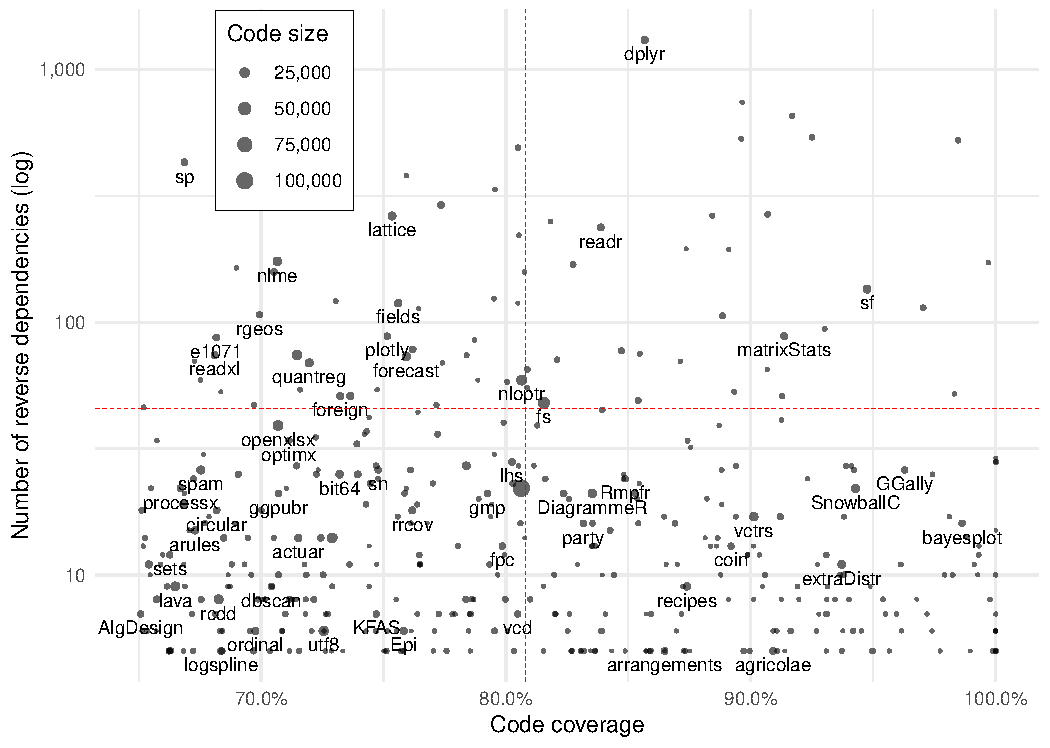
\includegraphics[width=.98\linewidth]{plots/corpus.pdf}
  \caption{Corpus overview}\label{fig:corpus}
\end{figure}

These packages come from the Comprehensive R Achive Network
(CRAN\footnote{\url{http://cran.r-project.org}}), the largest repository of
R code with over \AllCranRnd packages\footnote{CRAN receives about 6 new
  package submissions a day~\cite{Ligges2017}} containing over \AllRCodeRnd
and \AllNativeCodeRnd R and native code respectively. Unlike other open code
repositories like GitHub, CRAN is a curated repository. Each submitted
package must abide to a number of well-formedness rules that are
automatically checked asserting certain quality. Most relevant for this work
is that all of the runnable code (including code snippets from examples and
vignettes) is tested and only a successfully running package is admitted in
the archive.

We have downloaded and installed all available CRAN packages. Out of the
\AllCranRnd packages, we managed to install \AllLoadableRnd. The main reason
for this is that \rdt is based on R 3.5.0 and some of the packages are no
longer compatible with it. Some packages also require extra native
dependencies which were not present on our servers.  We have two criteria
for including a package into the corpus:
\begin{inparaenum}[(1)]
\item have runnable code that covers significant part of the package source
  code from which type signatures could be inferred, and
\item have some reverse dependencies that allows us to evaluate the inferred
  types on runnable code from these dependent packages.
\end{inparaenum}
The concrete thresholds were set to at least \ThresholdCodeCoverage of
expression coverage and at minimum \ThresholdRevdeps reverse dependencies.

The code coverage was computed for each package using
\covr\footnote{\url{https://github.com/r-lib/covr}}, the R code coverage R
tool.  The reverse package dependencies were extracted from the package
metadata using builtin function.

%
%
%
\section{Left overs}

SOME OF THIS STUFF CAN BE USED IN THE EVALUATION

%
%
\subsubsection{Possibly-NA Primitives}

A common primitive usage pattern is related to the presence of NAs:
programmers explicitly check for NAs in primitive vectors, possibly
sanitizing them if they are present.  NAs complicate practically every
computation using primitive vectors, a fact that many programmers appear to
be acutely aware of. For instance, consider the code in
Figure~\ref{fig:na-example}.

\begin{figure}[htbp]
\begin{center}

\begin{lstlisting}
binom.profile <- function(x, n, ...) {
  xn <- cbind(x = x, n = n)
  ok <- !is.na(xn[, 1]) & !is.na(xn[, 2])
  x <- xn[ok, "x"]
  n <- xn[ok, "n"]
  ...
\end{lstlisting}

\caption{NA checking example from the \code{binom} package.}
\label{fig:na-example}
\end{center}
\end{figure}

The \code{binom} package is a popular R package for computing confidence
intervals for binomial experiments, and the \code{binom.profile} function
does so using the profile likelihood, the details of which are not relevant
here.  This code snippet highlights a data sanitization pattern appearing at
the beginning of the function: the programmer first binds the vectors into a
matrix (line 2), with one column for each of \code{x} and \code{n}, then
finds rows where both columns are not NA (line 3), then extracts non-NA
values and stores them into \code{x} and \code{n} respectively (lines 4-5).
Importantly, this process is entirely quiet, and the user of
\code{binom.profile} will not be notified if their data happens to contain
NAs, and the NAs will be silently ignored.  In reality, the presence of NAs
in data could signify some sort of data corruption, and quietly ignoring
issues in data could lead users (read: statisticians) to draw flawed
conclusions from erroneous data.

To combat this, we introduce a modifier on primitive types: the type
\code{^T} signifies that primitive type \code{T} might contain an NA value,
while \code{T} signifies that \code{T} is NA-free.  The NA-free case has a
shorter syntax as NA-free vectors are \AT{more common} than the alternative.
If the \code{binom} developers were to annotate arguments \code{x} and
\code{n} with such an NA-free type, \contractr will notify users when
\code{binom.profile} is called with NA-full values, rather than just quietly
ignoring them.

Note that when combining call traces involving \code{^T} and \code{T} types,
we subsume \code{T} types into \code{^T} types: if NA-free and NA-full
vectors are passed to an argument, then we say that the argument can handle
NA-full vectors.  This is equivalent to saying \code{T <: ^T}.

%
%
\subsubsection{Scalar Primitives}

Initial analyses of our data revealed that programmers \AT{often} use
scalars (as explicitly as they can, anyway), and often do high-level
dimensionality checks on their data.  To illustrate, consider the code in
Figure~\ref{fig:scalar-vector-example}.

\begin{figure}[htbp]
\begin{center}

\begin{lstlisting}
hankel.matrix <- function( n, x ) { 
### arguments
### n = a positive integer value for the order of the Hankel matrix
### x = an order 2 * n + 1 vector of numeric values
    ...
    if ( n != trunc( n ) )
        stop( "argument n ix not an integer" )
    if ( !is.vector( x ) )
        stop( "argument x is not a vector" )
    m <- length( x )
    if ( m < n )
        stop( "length of argument x is less than n" )
    ...
\end{lstlisting}

\caption{Scalar/vector example from the \code{matrixcalc} package.}
\label{fig:scalar-vector-example}
\end{center}
\end{figure}

The \code{hankel.matrix} function takes two arguments (as described in the
comment in the code), and returns a Hankel matrix, which essentially is a
matrix where the skew-diagonals have a desirable property.  The function
body has a number of interesting checks: on lines 6-7, \code{n} undergoes an
integer ``type check''; on lines 8-9, \code{x} undergoes a vector ``type
check''; on line 11, \code{n} is assumed to be a scalar, as if it were a
vector, the code \code{m < n} would essentially check \code{m < n[i]} for
each element in \code{n}, returning a vector of comparison results, and the
conditional of an if must be a scalar else R generates a warning.

These checks exemplify functionality that we would like to include in our
type annotation language, namely, we would like our type language to
differentiate between scalars and vectors.  To that end, we introduce the
following types into our type language: for some primitive type \code{T},
the user may modify \code{T} with a modifier \code{[]} to indicate that it
is a vector of \code{T}.  Perhaps surprisingly, we found that scalars
\AT{occurred more frequently} than vectors, and for that reason we chose the
shorter scalar type syntax as the default.  The NA-free modifier works as
expected: \code{^T[]} indicates a vector of \code{T} that is free of NAs,
while \code{^T} indicates a scalar which is not NA.
 
%
%
\subsubsection{Matrices}

Matrices represent another layer of complexity on top of vectorized
primitives.  Internally, matrices are simply vectors with class ``matrix''
and a \code{dims} attribute indicating matrix dimensions, and while not
codified in the language semantics, many internal functions will coerce
vectors to matrices automatically.  Relying on automatic coercion is unwise,
and many functions check to ensure that their arguments are matrices.  For
instance, consider the code in Figure~\ref{fig:matrix-example}.

\begin{figure}[htbp]
\begin{center}

\begin{lstlisting}
rowWeightedMeans <- function(x, w = NULL, rows = NULL, cols = NULL,
                             na.rm = FALSE, ...) {
  # - - - - - - - - - - - - - - - - - - - - - - - - - - - - - - - - - - - - -
  # Validate arguments
  # - - - - - - - - - - - - - - - - - - - - - - - - - - - - - - - - - - - - -
  # Argument 'x':
  if (!is.matrix(x)) {
    .Defunct(msg = sprintf("Argument 'x' is of class %s, but should be a matrix. 
    The use of a %s is not supported, the correctness of the result is not guaranteed. 
    Please update your code accordingly.", sQuote(class(x)[1]), sQuote(class(x)[1])))
  }
  ...
\end{lstlisting}

\caption{Matrix example from the \code{matrixStats} package.}
\label{fig:matrix-example}
\end{center}
\end{figure}

The \code{rowWeightedMeans} function calculates the weighted means of rows
or columns of a matrix \code{x}.  This function exhibits good practice in
type checking arguments, rightly producing a message to the user indicating
that an explicit matrix should be passed.

To capture cases like this, we include a \code{class<matrix>} type in our
type annotation language.  If \code{rowWeightedMeans} were outfitted with
such a type, \contractr can perform the check present in this code
automatically, notifying the users passing ill-typed arguments.

%
%
\subsubsection{Forgoing Dimensionality} 

Thus far we've seen instances where we introduce types that subsume existing
argument validation code, but our intention is not to subsume {\it all} such
code.  As an example of something we {\it do not} want to do, consider the
code in Figure~\ref{fig:general-validation-example}.

\begin{figure}[htbp]
\begin{center}

\begin{lstlisting}
rowWeightedMeans <- function(x, w = NULL, rows = NULL, cols = NULL,
                             na.rm = FALSE, ...) {
  ...
  n <- ncol(x)
  if (length(w) != n) {
    stop("The length of argument 'w' is does not match the number of column in 'x': ", 
    length(w), " != ", n)
  }
  ...
\end{lstlisting}

\caption{General dimensionality check example from the \code{matrixStats} package.}
\label{fig:general-validation-example}
\end{center}
\end{figure}

This code is from later in the same \code{rowWeightedMeans} function
discussed previously.  Here, the length of the weights vector \code{w} is
being checked for equality with the number of columns in the matrix
\code{x}.  Specifying this relationship as a type amounts to {\it dependent
  typing}, which we believe too complex to retrofit onto a dynamic data
science language such as R.  Ultimately, we decided to leave these kinds of
checks up to the programmer.  

%
%
%
%
%
\subsubsection{Relationship Between Lists and Vectors}

The ease with which vectors may be transformed into lists is perhaps
indicative of a relationship between the two.  In R, all vectors can be
converted to lists with a simple call to \code{as.list}, and lists to
vectors with \code{unlist}, though care must be taken when unlisting a
non-homogeneous list, as coercions will be performed where possible, and the
function will simply do nothing if coercion is impossible.  That said, lists
and vectors have different access syntax, so vectors cannot stand-in for
lists without the \code{as.list} call above.

In sum, we opted not to include a subtyping relationship between vectors and
lists, keeping both types separate.  In practice, \AT{how often do \code{T[]
    | list<T>} types occur?}.  During our evaluation we also found it rare
that programmers would attempt to pass list-typed values to vector-typed
arguments and vice versa, and we will discuss this further in
Section~\ref{sec:evaluation}.

%
%
%
\subsubsection{Structs}
\label{subsec:structs}


We observed the use of consistently-named lists in \AT{a number of
  functions}.  In R, ``fields'' of named lists can be accessed using the
\code{$} operator, as illustrated in the code snippet in
Figure~\ref{fig:struct-ex}.

\begin{figure}[htbp]
\begin{center}

\begin{lstlisting}
agricolae::cv.model <- function(x) {
  suma2 <- sum(x$residual^2)
  gl <- x$df.residual
  promedio <- mean(x$fitted.values)
  return(sqrt(suma2/gl)*100/promedio)
}

data(sweetpotato)
model<-aov(yield~virus, data=sweetpotato)
cv.model(model)
\end{lstlisting}

\caption{Struct example from a test in the \code{agricolae} package.}
\label{fig:struct-ex}
\end{center}
\end{figure}

In the code snippet, the function \code{cv.model} takes an argument
\code{x}, which we observed to always be a {\it linear model}, which is part
of R's built-in statistics functionality.  Internally, linear models are
represented as lists with named elements, and one may access these named
elements using the \code{$} syntax, as seen on lines 2-4 in the snippet.  To
describe these kinds of values, we included a struct type in our type
system, allowing users to specify name, type pairs as part of list type
definitions.

Unfortunately, the inclusion of structs complicated our analysis by
polluting the data, illustrated on line 8 with the call
\code{data(sweetpotato)}.  It is quite common for R example code to use some
built-in data sets, such as \code{sweetpotato}, to show off some package
functionality with ``real data''.  When \typetracer is configured to detect
structs we saw a marked increase in misrepresentative types, as the types of
functions which use these data sets (such as \code{aov} in
Figure~\ref{fig:struct-ex}) became polluted with the names from the example
sets.  We implemented a unification strategy for struct types, removing them
if they co-occurred with list types, and turning them into lists if two
co-occurring struct types shared no common names, but even so we found
ourselves with function signatures that were full of noise introduced by the
struct names.

We still believe struct types to be useful to R programmers, and so our
language supports the type and \contractr will check them, though we
configured \typetracer to ignore them as they made the data substantially
less useful.  On the positive side, we found that \AT{get the number, but
  often} structs-typed values had a {\it class}, which helped motivate our
inclusion of class-like types in our type annotation language.  Classes are
discussed in more detail in Section~\ref{subsec:classes}.

%
\subsubsection{Data Frames}

One of the most popular classes in R is the \code{data.frame} class \AT{we
  have numbers here, grab em}.  Data frames and the derivative \code{tibble}
(from the \code{tidyverse} ecosystem) and \code{data.table} (from the
\code{data.table} package) types underpin a huge amount of data analysis in
R.

One way to deal with data frames is through the struct type, with a named
field for each column of the data frame, but as mentioned previously structs
introduced undue noise into \typetracer's analysis results.  Further
complicating data frames is that many functions built to operate on them
operate in a name-agnostic way.  For instance, the \code{tidyverse} package
ecosystem allows programmers to pass column names to functions which operate
on their data frames.  In base R, idiomatic data frame use is to use string
column names to select rows from the frame (unless only a single column is
of interest, wherein the \code{$} syntax is appropriate).  We include some
examples in Figure~\ref{fig:data-frames-bad} to illustrate the complexities.

\begin{figure}[htbp]
\begin{center}

\begin{lstlisting}
data(cars)

# tidyverse: Filter rows where speed is > 20. 
fast_cars_tidy <- filter(cars, speed > 20)

# base R: Get all rows where the "speed" column has a value > 20.
fast_cars_base <- cars[cars[, "speed"] > 20, ] # base example

\end{lstlisting}

\caption{Select examples of idiomatic \code{data.frame} use.}
\label{fig:data-frames-bad}
\end{center}
\end{figure}

Doing justice to this type will be an endeavour in and of itself, requiring
reconciliation of base R's \code{data.frame}, \code{tidyverse}'s
\code{tibble}, and \code{data.table}'s \code{data.table}.  Developing useful
types for the \code{tidyverse} ecosystem may well involve

It will also require proper treatment of function types, and perhaps even
parametric types, which dynamic analyses such as \typetracer are unable to
discern soundly.

In the context of our type annotation language, we will ascribe the type \code{class<data.frame>} to \code{data.frame}-typed values.
A more in-depth discussion of class types follows.

%
%
%
%
\subsection{Classes in R}
\label{subsec:classes}

As discussed in Section~\ref{sec:R}, the R runtime has more than one notion
of type.  The classes of function arguments are used by R as part of its
dispatch mechanism, the most prevalent of which (\AT{we have that number,
  too!}) is S3 dispatch, in which R dispatches on the (S3) class of the
first argument to a function, selecting the appropriate method to call for
the class.  To quickly illustrate, consider the code snippet in
Figure~\ref{fig:dispatch-ex}.

\begin{figure}[htbp]
\begin{center}

\begin{lstlisting}
# Quick example of S3 dispatch.
\end{lstlisting}

\caption{S3 dispatch in R.}
\label{fig:dispatch-ex}
\end{center}
\end{figure}

Classes are very prevalent in R \AT{number}, and so we include a
\code{class<class-name>} ... \AT{todo} \typetracer was outfit to report the
class of values, but some care needed to be taken so as to not overreport
class types, as {\it all} values have a class in R.  The main classes we
were interested in were matrix, array (higher dimensional matrices), and
data.frames, in addition to any user-defined classes.  In many cases
\AT{number?}, values with a user-defined class are in reality lists with
named elements, or structs.  Including class types, and having \typetracer
report them in place of structs, significantly reduced the noise in the
analysis and allowed us to gather more focused data.  To get a sense for
this difference, consider the code in Figure~\ref{fig:class-vs-struct}.

\begin{figure}[htbp]
\begin{center}

\begin{lstlisting}
# Example of gross struct that turns into class.
\end{lstlisting}

\caption{S3 dispatch in R.}
\label{fig:class-vs-struct}
\end{center}
\end{figure}

When set to ignore classes, \typetracer reports \AT{type} as the type of the function, as compared with \AT{other type} when configured to report classes.

%
%
\subsubsection{Multi-Classes}

A value can have multiple classes in R.  This is common practice in the
\code{dplyr} package, which extends the functionality of data frames: a
\code{data.frame} that passes through \code{dplyr} functions gains two
additional classes (\code{tbl} and \code{tbl_df}), bringing the total to at
least 3, in addition to whichever other classes that data frame happened to
have.  Note that when looking to perform S3 dispatch, R will try to match
{\it any} of the classes of the first argument to a dispatched function, so
each of these classes are important.

We found these so-called multi-classes to be surprisingly common, making up
\AT{occurrence} of the occurrences of class-typed values.  One possible
reason for this is that values can gain classes quite easily (e.g. the
\code{dplyr} example discussed above), somewhat polluting the output of
\typetracer.  Nevertheless, we found \AT{number} of occurrences of
monomorphic multi-class arguments, meaning that the function was always
called with a multi-class value in that argument position.

In the end, we support these multi-class types by allowing \code{class<...>}
types to contain a list of class names, so for instance a \code{dplyr}
\code{tibble} would have type \code{class<data.frame, tbl, tbl_df>} in our
type language, and when performing related contract assertions \contractr
will check that the value has every class that make up its type.

%
%
\subsubsection{Forgoing R's Object Systems}

R has multiple, disparate object systems, with the language providing direct
support for S3, S4, and R5.  Thus far, we've mainly discussed S3 and its
dispatch mechanism, and indeed our class types roughly capture the S3
classes of values.  We will not discuss R5 as it is still under development.

For S4, we have an \code{s4} type to denote S4 values, though we did not
elaborate on this type, and in practice S4 values have a class, and thus a
\code{class<...>} type.  We stuck to simple class-based types for S4 since
doing anything more would be immensely complicated, and outside of the scope
of this work.  For instance, the mechanics of S4 dispatch are more complex
than for S3 (S4 dispatches on the class of {\it all} arguments), and users
can define their own class hierarchies that we would need to incorporate in
our type analysis and contract checking frameworks.  Further, \AT{we found
  limited use of S4 during our analysis}, with S4 types being heavily used
in a select subset of packages (\AT{such as ...}), some of which make heavy
use of R's metaprogramming capabilities.  Coming up with a type system that
accounts for all of these factors and consolidates multiple
object-orientation frameworks in a single language design is an interesting
problem in and of itself, and we aim to extend our type annotation framework
to account for this in future work.  For now, S3 types suffice: S3 is the
most common object system in R, with no sophisticated hierarchies, and its
semantics are simple enough to be captured by our proposed design.

%
%
\section{Evaluation}
\label{sec:evaluation}

To evaluate the effectiveness of our type annotation language and contract
checking framework, we conducted a large-scale experiment based on the
corpus of 412 packages we used to inform our language design.  This corpus
represents some of the most widely used and thoroughly tested R libraries on
CRAN.

We configured \typetracer to infer the types of each of the functions that
are visible to package clients.  Recall that \typetracer's primary function
is to collect call signatures from observed function calls, and we ran
\typetracer on the test, example, and vignette code of all packages in the
aforementioned corpus.  These call traces were consolidated into a single
function type for each visible package function: \typetracer employs
unification strategies discussed in Section~\ref{sec:typesystemdesign} to
keep the size of signatures in check and only generates an \code{any} type
when missing and unused arguments were recored, and when a longjump caused
function execution to abort prematurely.  The types generated by \typetracer
will be analyzed in more depth in Section~\ref{subsec:stats}, and a
large-scale evaluation of the quality of these types will be discussed in
Section~\ref{subsec:eval}.

%
%
%
%
\subsection{Language Statistics}
\label{subsec:stats}

\subsection{Is our simple type language expressive enough to type R code?} Functions in
R can support arguments of multiple types by reflecting on the type to
perform appropriate conversions and computations. On the one hand, this form
of ad-hoc polymorphism makes R functions expressive; on the other hand, it
requires support for polymorphism in the typing scheme, making the type
system complex.  Our system lacks explicit support for
polymorphism. Instead, it supports union, any and ... types. A union type is
inferred when values of multiple types are observed at a function parameter
and return position, any type is inferred when an argument is missing or
unused, and ... is inferred for vararg parameters. Furthermore, list element
types can be inferred as any if they have more than 5 different types. Values with many different types can result in
a large number of alternatives in the type inferred for that position,
making it hard to read and unwieldy for end-users. To evaluate this
''expressivity gap`' between our type inference scheme and R functions, we
look at the number of different types in the parameter and return types of
the XXX functions in our corpus.

\begin{figure}[!h]  \centering
  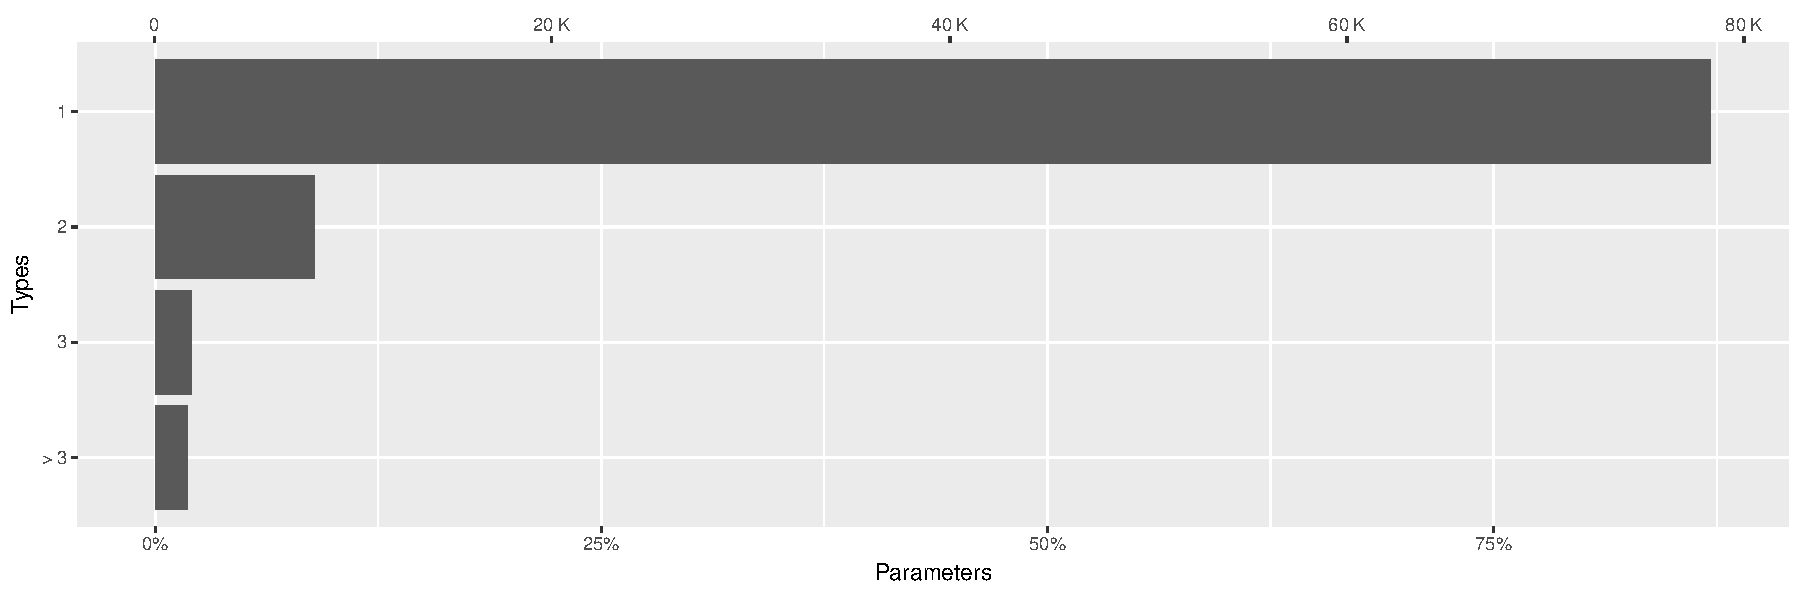
\includegraphics[width=\linewidth]{plots/union_frequency.pdf}
  \caption{Types inferred for each position}\label{fig:unionfreq}
\end{figure}

We observe that XXX% of the positions have a single type ascribed to them. XXX%
have five or more types ascribed to them. Parameter PARAMNAME of function
XXXXCOLONCOLONXXX has the maximum, XXX, types ascribed to it. This implies that
most functions admit or return a uni-typed value.

Figure XXX shows ten most common type categories that occur by themselves. We
observe that three scalar types, double, logical, and character are most
frequent. This is followed by XXX vararg parameter positions. Next, XX% of the
parameter types are any because arguments at those positions were either missing
or unused in at least one call to those functions. Together, these types amount
to more than 50%. This is followed by double vector, the unit type, null,
character vector, and classes matrix and data.frame respectively.

Figure 1 shows the number of alternatives in the inferred type of function
parameter and return values.

XXX\% of the parameter positions are monomorphic. 
\typetracer observes XXX calls to XXX functions with XXX arguments. This
translates to XXX parameters and XXX return types. 
A parameter or return type is  from unioning all the distinct observed types of 

Figure 1 shows the distribution of parameter and return types for these
functions.


class is the most common type in our corpus, accounting for XXX% of all the
inferred types. This is followed by an almost equal proportion,
28%, scalar types and, surprisingly, only 13% vector types. Vectors are the
workhorse of R, most primitive operations in R are vectorized and literals are
treated as single element vectors. It is unexpected to observe twice as many
scalars as vectors. It is even more unexpected to observe class as the most
common type. class of an object is used for dynamic dispatch by the S3 object
system in R. This suggests that usage of S3 is prevalent in our corpus.



null types. Together, these four types make up for 80% of the observed types in
our corpus.
The other types, occurring only XXX% of the times include XXX environment types,
XXXX expression types, XXXX pairlist types and lastly, XXX externalptr types.




We analyzed the type signatures generated by \typetracer in order to build
up a profile of our type annotation language.  We were interested in broad,
high-level information, such as the distribution of generated types, the
level of polymorphism observed in the types, and the distribution of sizes
of union types.

%
%
\subsubsection{Type Distribution}

\AT{Include a figure? Histogram(s) of types?}

In order to count the occurrences of each type, we subdivided them into {\it kinds}: 
For our purposes, the {\it kind} of a type is equivalent to it's top-level type constructor, so all classes have kind ``class'', all lists have kind ``list'', and so on.
We found that classes are the most common kind of type, accounting for roughly 31\% of types.
\AT{Make sure to transform class<function> into any=>any.}
In order, the most common classes are matrices (12\%), data.frames (7.5\%), formulas (2\%), factors (2\%), and tibbles (2\%).
Roughly 25\% of classes are part of R's base language implementation, the others being defined as part of some package's functionality.

Besides classes, scalars and vectors are the next most common kind, making up 41\% of types. with scalars making up 28.1\% of types and vectors 12.65\%.
Nulls and lists follow at 8\% and 7\% respectively, and the vararg type \ldots makes up 6.5\% of arguments.
This all totals up to over 90\% of types.
We will discuss the any type in more detail in Section~\ref{subsec:any}.

It would appear that our simple type annotations nicely account for the landscape of values in R.
\AT{Not sure what to say about classes.}
% Classes are a common kind of type in R, and for the purposes of this type annotation language allowing users to specify class names as part of class types is welcome: we saw that the breakdown of the class kind does not reveal many outlier classes,

%
%
\subsubsection{Polymorphism}

The polymorphism in R is best described by {\it ad hoc} polymorphism, wherein polymorphism is implemented by function and operator overloading (see S3 dispatch) rather than in some more fundamental way in the language design.
For the purposes of this evaluation, we will say that an argument is polymorphic if its type is a union of two or more types, in other words the argument has been observed to take more than one type of value.

\AT{We need better numbers on this.}
We found that 15\% of argument positions were polymorphic, and that X\% of functions were polymorphic.

Our type annotation language does not support sophisticated class typing, and much of the polymorphism in R is due to these classes, namely through the S3 dispatch mechanism. 
In future work, we aim to more fully handle S3 and objects in R.
For now, if we count out 

%
%
\subsubsection{Size of Union Types}

%
%
\subsubsection{Use of \code{any}}
\label{subsec:any}

%
%
%
%
\subsection{RQ2: How good are type signatures generated from traces?}
\label{subsec:eval}

\AT{Me}

In the last section, we evaluated our type annotation language based on a set of function types that were automatically generated by \typetracer.
Now, we're interested in knowing how representative our trace-generated types are of the functions they were generated for.
To measure this, we conducted a large-scale experiment: for each package in the corpus discussed in Section~\ref{sec:corpus}, we ran \typetracer on its test, example, and vignette code, obtaining types for package functions, and then subsequently ran the test, example, and vignette code of each of the package's reverse dependencies (or clients).
We collected failed contract assertions in order to analyze them and perhaps identify weaknesses in our type annotation language.

%
%
\subsubsection{Overall Results}

We ran our evaluation on \NUMPKGSEVAL packages and recorded \NUMASSERTIONS total assertions.
Overall, we found that only \PERCFAILEDASSERTIONSWUNDEF of contract assertions failed.
We made a simplification in our analysis, capping the number of function arguments we generate types for to 20, and this resulted in only \PERCASSERTIONSUNDEF failed assertions, which suggests that the simplification we made did not greatly affect the results.
Once we controlled for these, we found that \PERCFAILEDASSERTIONS of all assertions failed for reasons related to our generated types.
Additionally, we found that \PERCSUCCARG of parameter types and \PERCSUCCFUNS of functions types were never violated.
The number of immaculate function types increases to \PERCSUCCFUNNOSTHREE if we count out S3 functions:
These S3 functions represent user-defined polymorphism which we do not tackle in this work.
Overall, these numbers are promising, and suggest that the type signatures generated by running \typetracer on our corpus are indeed representative, and capture intended function behaviour.

%
%
\subsubsection{Breakdown of Contract Assertion Failures}

We breakdown the failed assertions by type in Table~\ref{tbl:fail-breakdown-0}.
By far the most commonly failed assertion is one asserting that a value with ${\bf dbl}[]$ type has type ${\bf class}\langle matrix \rangle$.
This was a deliberate design decision, as coercion from vectors to matrices is ad hoc at best, and surely not a practice codified in the language.
In a similar vein, another popular failing assertion is checking if a ${\bf dbl}[]$ has type ${\bf int}[]$, another case of commonly performed coercion.
We did not include these types of coercions in our type annotation framework as programmers cannot rely on them, and it is not always the case that the coercions are safe to perform. 

\begin{table}
% BEGIN Autogenerated

\begin{tabular}{llrrr}
\toprule
Actual Type & Expected Type & \# Failed Assertions & \% Total & Cumulative \%\\
\midrule
double[] & class<`matrix`> & 371896 & 27.37 & 27.37\\
double[] & integer[] & 117212 & 8.62 & 35.99\\
character & class<`bignum`> | raw[] & 100100 & 7.37 & 43.36\\
double & integer | null & 60570 & 4.46 & 47.81\\
double[] & class<`timeSeries`> & 58872 & 4.33 & 52.15\\
\addlinespace
class<matrix> & class<`timeSeries`> & 55005 & 4.05 & 56.19\\
double[] & double & 53338 & 3.92 & 60.12\\
double & class<`data.frame`> & 32553 & 2.40 & 62.51\\
double[] & class<`data.frame`> & 31576 & 2.32 & 64.84\\
double & integer & 20586 & 1.51 & 66.35\\
\bottomrule
\end{tabular}
% END Autogenerated
\label{tbl:fail-breakdown-0}
\caption{Top types of contract assertion failures.}
\end{table}

In addition to the raw number of failing contract checks, we were interested in how many functions had a parameter where a contract check failed.
Overall, we found that \PROPFUNSFAILEDCHECK of functions had a failing contract check.
Digging a little deeper, we noticed that many of these functions were performing S3 dispatch, which is part of R's object-orientation framework which we will tackle in future work.
Removing those functions, we see that \PROPFUNSFAILEDCHECKNOSTHREE of functions exhibited failing contract checks.
These are functions which were under-tested, as calls to these functions represent only \PERCCALLSBADFUNSINTESTS of recorded calls during \typetracer's run on the core corpus to infer types.

Turning our attention now to arguments, we found that only \PROPARGSFAILINGASSERTS of function parameters exhibited a failed assertion.
Table~\ref{tbl:fail-breakdown-0} showed the raw results from counting runtime occurrences, but that data alone does not tell the full story, as some failures may be overrepresented if e.g. a failing contract assertion was in a loop.
We were interested in a breakdown of type signature by parameter, and seeing how often those contracts were violated.
Table~\ref{tbl:fail-breakdown-1} breaks down the results from Table~\ref{tbl:fail-breakdown-0} by parameter position, folding away multiple identical failed contract assertions for the same parameter position.
The first row of this table reads: a value of type ${\bf chr}[]$ was passed to 183 different argument positions expecting a value of type ${\bf chr}$, representing 2.05\% of all arguments where a contract check failed.

The main takeaway from Table~\ref{tbl:fail-breakdown-1} is that there appear to be no pathological kinds of failing assertions: programmers are not disproportionately passing values of one type to arguments expecting values of another.
In other words, our type language appears to match with programmer intuitions: had we failed to account for a key, type-based assumption that R programmers make, we would see it at the top of the table.

 \begin{table}
% BEGIN Autogenerated



% END Autogenerated
 \label{tbl:fail-breakdown-1}
 \caption{Most common failing contract checks by type. Note that for this table, we collapsed multiple identical failed assertions into one, meaning that single arguments with multiple (identical) failed assertions are only counted once.}
 \end{table}

%
%
% \subsubsection{Patterns in Failed Contract Assertions}

% While Table~\ref{tbl:fail-breakdown-1} revealed no glaring patterns in failed assertions, there are a few subtle issues that we will discuss.
% First, \PERCFAILEDVECTOSCA of failed checks broken down by parameter position failed due to vectors being passed where scalars were expected.

% We observed an interesting corner case and quirk of R in looking at functions with values that default to NA.
% In R, recall that there is a different type of NA for each primitive, and when the literal value \code{NA} appears in code, R assumes it to be the logical NA.
% For the purposes of our analysis, this has the effect of introducing $\string^{\bf lgl}$ types where they (probably) don't belong, particularly when programmers fail to effectively test their code.
% For example, a function header like \code{function(x, y=NA)} will have $\string^{\bf lgl}$ as part of the type of parameter \code{y}.
% We tried to control for this in our analysis, and indeed $\string^{\bf lgl}$ is a subtype of all NA-able numeric types.



%
%
%
%
\subsection{Usefulness of the Type Checking Framework}

\section{Conclusion}

\ldots


\bibliography{bib/biblio,bib/jv,bib/r,bib/new,bib/gradual}
\end{document}
